\chapter{Length of Stay Classification Using Supervised Learning}
  \label{chap:classification}

In order to use a supervised learning algorithm to identify objects with
a particular classification, we first need \textit{feature vectors} to
describe these objects. In our case, each patient is converted into one
feature vector, where each \textit{feature} in this vector tells us
something about the
patient that can help us decide which LOS category he or she should be
placed in. The features comprising each feature vector must be the same,
but with different values. By comparing feature values between different
vectors, we are able to decide which \textit{class} or category a patient
belongs in. For example, if we wanted to classify the weather on a given
day as ``good'' or ``bad'', we could use two features -- temperature and
the amount of rain -- which are likely to be key indicators. Classifying
several days simply involves creating a feature vector that corresponds
to each day, with differing values for the temperature and the amount of
rain, and using these values to decide whether or not a day had good or
bad weather.

Since we will be using supervised learning techniques, we need
\textit{training examples}, which consist of a set of feature vectors
that are already labelled with the class that it belongs in. These
training examples are then used by a classifier to ``learn'' the
relationship linking the feature vectors to their class labels. Once we have
``trained'' the classifier to learn this relationship with the pre-labelled
data, it will then be able to predict the class of any feature vector that we
give it.

In this
chapter we describe each of the learning algorithms we used to model the
relationship between the feature vectors and the LOS.

\section{Zero-R and 1R}
\label{sec:zeror}
Short for ``0-rule'' and ``1-rule'' respectively, Zero-R and 1R are
very simple classifiers. Zero-R uses no features to predict the class, and
1R only uses one.

Given a data set, the Zero-R classification algorithm will find the class that
occurs the most often, and predict this class for all new examples. For LOS
classification, if one class in a data set was ``LOS $\leq$ 2 days'' and
the other was
``LOS $>$ 2 days'', and feature vectors (which represent patients in this
scenario) were more commonly labelled ``LOS $\leq$ 2 days'', then Zero-R will
predict all unseen patients with ``LOS $\leq$ 2 days''.
The prediction decision of Zero-R is very easy to understand,
and its results also provide an apt baseline for evaluating the more
sophisticated classifiers used in this work.

1R works by considering each feature individually.
For each of the values of the
feature, 1R finds the class with the highest frequency and creates a rule
from this observation. If the feature is numeric (that is, its values are
continuous rather than discrete), then 1R will partition the spectrum of
values into discrete buckets. This is known as \textit{discretisation}.
The error rate, expressed as the ratio of correct predictions to the total
number of examples in the data set,
is calculated for each rule that is generated
in this way. The rule with the lowest error rate is then chosen as the 1-rule
for this classifier,
and if there is a tie, it is broken randomly. As with Zero-R, the prediction
decision of 1R is transparent and it provides another baseline upon which
more sophisticated classifiers can be evaluated. Studies have also found that
1R performs quite well in terms of accuracy relative to other classifiers
\cite{Holte1993}.

Concretely, given a feature
vector of the form \textit{(age, gender, has\_cancer)},
1R will split the ages of
all patients into discrete categories
(such as \textit{0-20, 21-40, 41-65, 66+}). It
will then check the class labels for all training examples in the data set
that have \textit{age} in the 0-20 category
(as that is the first value for the discretised \textit{age} feature) and
note the most common class, proceeding similarly for the rest of the
categories of \textit{age}. Then it will consider \textit{gender}, which has
two possible values $\{$\textit{male, female}$\}$, and finally \textit{has\_cancer}
with two values $\{$\textit{true, false}$\}$. This results in 8 rules,
corresponding to three features.
An example of a rule is that \textit{age 0-20} most commonly
has ``LOS $\leq$ 2 days''. For each of these rules, 1R will attempt to
use only that rule to predict the LOS class for each example in the data set,
noting down the error rate. 1R then chooses the feature that produces rules
with the highest total accuracy.

\section{Na\"{i}ve Bayes}
Unlike 1R, which considers only one feature in the feature vector, Na\"{i}ve
Bayes (NB) classifiers allows all features to contribute equally to the
classification decision. Such classifiers apply Bayes' theorem with the
(unrealistic) assumption of independence between features, hence the
description \textit{na\"{i}ve}. This means that we
calculate the probability that a particular feature value belongs in a class
without considering the effect of other features on this probability. This
probability can be computed by
counting the frequency with which the value is associated with a class in the
training data. After these probabilities are computed, classifying a feature
vector simply involves multiplying the probabilities of each feature belonging
to each possible class. The predicted class for that feature vector is then the
class with the highest probability.

Speaking mathematically, Bayes' theorem states that:
\begin{equation*}
\mathbb{P}(Class_i|F_1,F_2,\ldots,F_n) =
  \dfrac{\mathbb{P}(F_1,F_2,\ldots,F_n|Class_i)\mathbb{P}(Class_i)}{\mathbb{P}(F_1,F_2,\ldots,F_n)}
\end{equation*}
Since we assume that the features are independent, we can simplify the above as:
\begin{equation*}
\mathbb{P}(Class_i|F_1,F_2,\ldots,F_n) =
\dfrac{\mathbb{P}(F_1|Class_i)\mathbb{P}(F_2|Class_i)\ldots \mathbb{P}(F_n|Class_i)\mathbb{P}(Class_i)}{\mathbb{P}(F_1,F_2,\ldots,F_n)}
\end{equation*}
This gives us the probability that the feature vector $(F_1,F_2,\ldots,F_n)$
belongs in the $i$-th class. Classifying the feature vector involves
calculating this probability for each for each class and choosing the class
with the highest probability.

Since we compute the probability of each feature value belonging in a
particular class by counting the frequency of each value's occurrence with
respect to the class, it is sometimes possible that a feature value has zero
probability of being in a certain class. This would make the numerator of the
above equation zero. A feature vector that could otherwise have been highly
likely to belong in class $i$ is now counted as having zero probability of
belonging in the class. In order to ensure that each probability is non-zero,
a small constant is added to all probabilities in a process called
\textit{Laplace smoothing}, which is commonly used for NB classifiers.

Like 1R, numeric features also need to be handled separately from nominal ones.
The typical approach is to assume that the values of a numeric feature follow a
normal (or Gaussian) distribution with mean and standard deviation calculated
from the values that the feature takes with respect to each class.
This allows us to use the probability
density function of the normal distribution to calculate the probabilty of the
feature belonging to a particular class:
\begin{equation*}
\mathbb{P}(F_i=x_i|Class_i) =
  \dfrac{1}{\sqrt{2\pi}\sigma}e^\frac{(x_i-\mu)^2}{2\sigma^2}
\end{equation*}

Despite the na\"{i}ve independence assumption of the NB classifier, it often
works surprisingly well in practice and is relatively fast to train. We use it
in our work both as a simple classifier in its own right, and also as a more
sophisticated baseline to Zero-R and 1R.

\section{C4.5 Decision Tree}
\label{sec:c45}
Decision trees (DT) can be specified recursively and are an example of a
``divide-and-conquer'' approach to learning. First, we choose a feature to
place at the root node and then create one branch for each possible value.
This partitions the data set into subsets, one for every value that the
feature takes. We repeat this for each branch, choosing different features
each time and continuing to divide the data set into progressively smaller
subsets, growing the tree.
If all examples in a subset have the same class at any point during
this process, we stop splitting that subset.

The only thing left to specify
now is how to decide which attribute to split on. Note that when splitting,
we would like to create subsets that are as ``pure''
-- that is, containing as many
instances of the same class -- as possible, so that the splitting may
terminate earlier. Since we would like our trees to be as small as possible to
prevent overfitting and allow the best generalisation ability,
we would therefore like to choose the feature to split on such that the
created subsets were as pure as possible. The measure of purity used in
learning decision trees is the \textit{information}, and is measured in
\textit{bits}. At any node (or subset) of the tree, this measure represents
the expected amount of information that would be needed to classify a new
example, given that the example reached the node. The information at each
node is calculated using the \textit{entropy} function:
\begin{equation}
\label{eqn:entropy}
\mathrm{entropy}(p_1,p_2,\ldots,p_n) = -p_1\mathrm{log}p_1 -p_2\mathrm{log}p_2 \ldots -p_n\mathrm{log}p_n
\end{equation}
Given $k$ classes, $c_1,\ldots,c_k$ is the number of instances in each
class at a node, and $\sum_{i=1}^k c_i = c$ is the total number of instances
at that node, the information of that node is then:
\begin{equation*}
\mathrm{info}(c_1,\ldots,c_k) = \mathrm{entropy}\left(\frac{c_1}{c},\frac{c_2}{c},\ldots,\frac{c_k}{c}\right)
\end{equation*}

To find the attribute to split on, we assume we are splitting on a particular
attribute, and calculate the information at the node given the split. We do
this for each attribute, and compute the \textit{information gain} from
splitting on that attribute:
\begin{equation*}
\mathrm{gain}(feature) = \mathrm{info}(\text{child node}) - \mathrm{info}(\text{parent node})
\end{equation*}
The feature that is chosen is therefore the one with the highest information
gain.

Decision trees are fast to train and produce models that are straightforward
for humans to interpret, the latter of which is particularly valuable in a
clinical environment. We will use the C4.5 tree induction algorithm, which is
considered the state-of-the-art and handles different types of feature values
as well as missing values.

\section{Logistic Regression}
Logistic regression (LR) is a regression technique used for when the dependent
variable is dichotomous or two-valued, and thus it is a suitable candidate to
use for our LOS classification problem.
Previous work on trauma LOS prediction by
Dinh et. al. \cite{Dinh2013a}, as well as many attempts at modelling the LOS
in various medical domains, have all used logistic regression, often as a
starting point.

For a class variable with two possible values that occur with
probability $p$ and $1-p$ respectively, and a feature vector
$(F_1,F_2,\ldots,F_n)$, the logistic regression model is:
\begin{equation*}
\begin{aligned}
\mathrm{logit}(p) &= \mathrm{log} \left(\dfrac{p}{1-p}\right) \\
  &= \beta_0 + \beta_1F_1 + \beta_2F_2 + \ldots + \beta_nF_n
\end{aligned}
\end{equation*}
For LOS classification, this can be rearranged to:
\begin{equation*}
\begin{aligned}
p &= \mathbb{P}(Class=\mathrm{LOS }\leq2\mathrm{ days}|F_1,F_2,\ldots,F_n) \\
  &= \dfrac{e^{\beta_0 + \sum^n_{i=1}\beta_i F_i}}{1 + e^{\beta_0 + \sum^n_{i=1}\beta_i F_i}}
\end{aligned}
\end{equation*}

Training the logistic regression classifier, then, is a matter of finding the
$\beta_i$ that will maximise the likelihood (conditional probability of the
data given the values for $\beta_i$) of the given data set. This is done using
numerical methods, where estimates of the $\beta_i$ are chosen, the likelihood
computed, and the $\beta_i$ are updated, and so on: this process is repeated
until parameter estimates converge or do not change more than a given threshold
value.

To classify a feature vector $\mathbf{x} = (x_1,x_2,\ldots,x_n)$, we substitute the
$x_i$ into the above equation in place of the $F_i$, which gives us a
probability. If this probability is above a particular threshold, then we
classify the example as belonging to the class ``LOS $\leq$ 2 days'', otherwise
it is classified as ``LOS $>$ 2 days''. Usually this threshold is 0.5.

\section{Support Vector Machine}
Support vector machines (SVMs) are an example of a supervised learning algorithm
capable of classifying training examples into two classes. They are one of the
best algorithms in terms of predictive accuracy \cite{Bellazzi2008}. Despite
this, they have not been widely applied to predicting the LOS, which gives us
an opportunity to evaluate their performance in our LOS classification problem.

Given a set of $n$-feature vectors, we can represent each vector as a point in
$n$-dimensional space, where each feature is a dimension. The SVM will try to
find a \textit{hyperplane} that separates the two classes. Usually there are
many such hyperplanes; the distinguishing aspect of an SVM is that it will
find the hyperplane that maximises the distance between the two nearest points
in each class. This distance is called the \textit{margin}, and the intuition
is that maximising it will give us the greatest possible separation between the
classes -- the classifier comes no closer to either class than it needs to.
This gives the SVM the best generalising ability to classify new examples.
\begin{figure}[h]
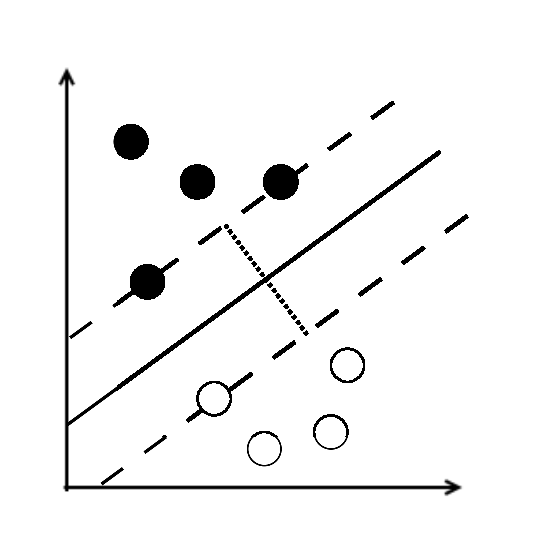
\includegraphics{images/method/svm-example.eps}
\caption{An example of a 2-dimensional SVM.}
\label{fig:svm}
\end{figure}

Figure \ref{fig:svm} shows an example of a two-dimensional feature space, with
two classes of points (black and white). We can see the hyperplane, in this
case a line since we are only in two dimensions, separating the two classes
with as much margin as possible. In
this case, the points are linearly separable: all white points lie on one side
of the hyperplane, and all black points lie on the other. In practice, this is
not common, and often data cannot be separated cleanly by a hyperplane.
Note that the points closest to the margin are those that are most likely to be
ambiguous when the data cannot be cleanly separated. The SVM will progressively
remove more and more of these ambiguous points from consideration when it
cannot find a hyperplane until it finds a suitable one.

Instead of removing points from consideration by the SVM, we can also specify
a \textit{kernel function}, which transforms the original feature space into
some other non-linear space. Commonly, polynomial functions of degree 2 or
greater are used, and theoretically they can approximate non-linear boundaries
between classes to any arbitrary accuracy. However, this is usually not
practically possible with data sets containing even a modest number of features
(around 10), due to the computational complexity of estimating a large number
of coefficients that are introduced by the transformation.

SVMs can be specified mathematically as a type of optimisation problem known
as \textit{constrained quadratic optimisation}. Given $m$ training vectors
$\mathbf{x_i} \in \mathbb{R}^n, i=1,\ldots,m$ and their labels
$y_i \in \{-1,+1\}, i=1,\ldots,m$, the optimisation problem can be written as:
\begin{equation*}
\begin{aligned}
& \underset{\mathbf{w},b}{\mathrm{minimise}}
  && ||\mathbf{w}|| + C\sum_{i=1,\ldots,m} s_i \\
& \text{subject to}
  && y_i(\mathbf{w}^T\phi(\mathbf{x_i})+b) \geq 1 \\
& && s_i \geq 0, i = 1,\ldots,m
\end{aligned}
\end{equation*}
where $\phi(\mathbf{x})$ is the kernel function, and
$\mathbf{w}\cdot\mathbf{x_i} + b = 0$ is the hyperplane that the SVM finds.
The $s_i$'s allow the SVM to ignore some examples if it cannot find a suitable
hyperplane, and $C$ (sometimes called the SVM's complexity constant) is a
constant specified by the user that controls how much we want to balance
finding the best possible margin with allowing misclassified examples.
Note that for a linear kernel, $\phi(\mathbf{x}) = \mathbf{x}$. Training the
SVM involves solving this optimisation problem and obtaining values for
$\mathbf{w}$ and $b$.

To classify an instance $\mathbf{x_{new}}$, we simply find the sign of
$\mathbf{w}\cdot\mathbf{x_{new}}+b$. This will tell us which one of the
two classes the new example belongs to.

\section{$k$-Nearest Neighbour}
In this section we will describe the $k$-nearest neighbour ($k$-NN) algorithm
and discuss some extensions which we use in our work. Additionally, we will
describe our contribution, which is an extension of the distance metric for
finding the nearest neighbours.

\subsection{Basic Algorithm}
The $k$-nearest neighbour classifier is an example of an
\textit{instance-based} learning algorithm. This is because it does not, unlike
the other classifiers described in this section, attempt to deduce or
generalise a relationship between the features and the class: it simply stores
all training examples and classifies an unseen example by finding the $k$
``nearest'' examples (or \textit{instances}) and assigning the majority class
to the new example. In the simplest form of the algorithm, $k$ is chosen to be
1 and the Euclidean distance is used to measure the closeness of neighbours:
\begin{equation*}
\mathrm{Distance} = \sqrt{(x_1-y_1)^2 + (x_2-y_2)^2 + \ldots + (x_n-y_n)^2}
\end{equation*}
where $x_i,y_i$ are the values of the $i$-th feature for two different feature
vectors (or instances).

Like the Na\"{i}ve Bayes classifier, $k$-NN allows all features to be taken
into account equally when classifying a new example. However, since feature
values often span different ranges and units of measurement, a particularly
large range of values for a feature would contribute much more to the distance
than another feature that spans a lower set of values.
To avoid this, it is important to \textit{normalise} the
values of each numeric feature before using $k$-NN: for each feature $i$, we
calculate the normalised value of the feature for each training example. This
is done using the following relationship:
\begin{equation*}
a_i = s\left(\dfrac{v_i - \mathrm{min }v_i}{\mathrm{max }v_i - \mathrm{min }v_i}\right) + t
\end{equation*}
where $a_i$ is the normalised value, $v_i$ is the actual value in the data
set, max $v_i$ and min $v_i$ are taken over all training examples, $s$ is a
scaling factor $t$ indicates how much to translate the range by. If $s=1$
and $t=0$, then the range of normalised values will be in $[0,1]$.

\subsection{Existing and Proposed Extensions}
There have been many extensions proposed to the $k$-NN algorithm described
above. These usually seek to find a more suitable distance metric for the
problem domain at hand, or to reduce the storage requirements of the original
$k$-NN algorithm. We will focus on two extensions to the Euclidean distance:
K* and our proposed distance function, Ranked Distance.

\subsubsection{K*: Instance-based Classifier with Entropic Distance Function}
Cleary and Trigg developed K*, an instance-based classifier that uses entropy
to measure the distances between instances \cite{Cleary1995}. They consider
the distance between two instances to be the complexity of transforming one
into another. Define a sequence of transformations on an instance:
\begin{equation*}
\bar{t}(a) = t_n(t_{n-1}(\ldots t_1(a)\ldots)), \bar{t} \in T
\end{equation*}
where $\bar{t} = t_1,\ldots,t_n$. We can define a probability function $p$
that gives the probabilities of these transformations occurring, and then we
can define a probability function that gives the probabilities of all paths
(transformations) from example $a$ to $b$:
\begin{equation*}
P^*(b|a) = \sum_{\bar{t}\in T:\bar{t}(a)=b} p(\bar{t})
\end{equation*}
Within this framework, we can define transformations for both real-valued and
categorical features, which allows K* to work with all types of features.
The K* function is then defined as:
\begin{equation*}
K^*(b|a) = -\mathrm{log}_2P^*(b|a)
\end{equation*}

To calculate the probability of an instance $a$ being in a class $C$, we sum
the probabilities from $a$ to each instance of $C$, and repeat for each class.
The predicted class will be the one with the highest probability:
\begin{equation*}
P^*(C|a) = \sum_{b\in C} P^*(b|a)
\end{equation*}

We use K* as a comparison to the basic NN algorithm and also as a comparison
to $k$-NN with our distance function.

\subsubsection{Proposed Approach: Ranked Distance}
\label{sec:rankeddist}
\paragraph{Intuition}
As we mentioned earlier, all features are considered equally in a $k$-NN
classifier, which implies that all features are equally important in predicting
the class. In practice, however, this is not always the case: to predict the
LOS of a trauma patient, the severity of their injury should affect the final
LOS more than whether or not they can speak English (which could be just two
of many features that are recorded about a patient). Our contribution is thus
a modified distance function to take the relative importance of attributes into
account. 

\paragraph{Mathematical formulation}
Given two instances $\mathbf{x} = (x_1,x_2,\ldots,x_n)$ and
$\mathbf{y} = (y_1,y_2,\ldots,y_n)$, the distance between them is given by:
\begin{equation*}
\mathrm{Distance} = \sum_{i=1}^n w_i |x_i-y_i|
\end{equation*}
where the $w_i$s weight the contribution of the $i$-th feature to the overall
distance that is computed by the $k$-NN algorithm. We assume that all feature
values have been normalised, as described above.

\paragraph{Assignment of weights}
The weights $w_i$ can be tuned to match the particular problem that is being
investigated. For our LOS classification problem, we will consider two ways
of weighting features:
\begin{enumerate}
\item The weight of each feature is the magnitude of the correlation
coefficient
between it and the class, meaning that features that are more highly correlated
with the class will contribute more to the distance. The correlation
coefficient $r_i$ for feature $i$ with the class $c$ can be computed by:
\begin{equation*}
r_i = \dfrac{\sum_{i=1}^m (x_i-\bar{x})(c-\bar{c})}{\sqrt{(\sum_{i=1}^m x_i-\bar{x})(\sum_{i=1}^m c-\bar{c})}}
\end{equation*}
where $m$ is the number of training examples, $x_i$ is the value of feature
$i$, and $\bar{x}$ and $\bar{c}$ are the arithmetic averages of the feature
values and the class values respectively. 
\item We compute the correlation coefficients as described in the point above.
This gives us a ranking of the importance of each feature to the prediction of
the class, with 1 being the highest rank (indicating the most importance) and
$n$ being the lowest rank (indicating the least importance).
Instead of using the values of the correlation directly to weight
the distance contribution of each feature, we specify a function:
\begin{equation*}
f : \mathrm{Rank} \rightarrow \mathbb{R}, \mathrm{Rank} \in \{1,2,\ldots,n\}
\end{equation*}
that describes
how the weights of the features vary with the rank. This function should
inituitively be non-increasing and should produce lower values when the rank
number is greater, meaning that less important features have a lower weight
in the distance calculation.
Note that choosing $f(\mathrm{Rank}) = k$ for any non-zero constant $k$
results in all features contributing equally to the distance calculation.

\noindent We will use $f(\mathrm{Rank}) = \frac{1}{\mathrm{Rank}^c}$, where
$c$ varies from 0 to 1.
\end{enumerate}

\section{Multi-layer Perceptron}
Multi-layer perceptrons (MLPs) are a generalised form of the
\textit{perceptron}, first
studied extensively by Rosenblatt \cite{Rosenblatt1962}. The original
motivation of the perceptron 
was to develop a very simple artificial neural network to model the
behaviour of neurons in the brain. The perceptron model for a two-class
problem is a linear combination of the features: that is,
$h(\mathbf{x}) = \sum w_i x_i$ where the $w_i$ are the weights of the model.
There is an input node, called a \textit{neuron}, for each feature, and the
weights are applied to the connections between these input neurons to the
output.
Usually, a constant term of 1 called the \textit{bias} is also added to the
model for an additional trainable input. To classify an item, we substitute it
into $h(\mathbf{x})$; if the value is above a particular threshold, we label it
as class 1, else it belongs in class 2. For convenience, we can let this
threshold be 0. Training the perceptron involves the following steps:
\begin{enumerate}
\item Start with random numbers for the weights $w_i$.
\item For each training example $\mathbf{x_i}$: calculate $h(\mathbf{x_i})$.
If it is correctly classified, do not update the weights.
If it is incorrectly classified, add a multiple of the misclassified
instance to the current weights using
$\mathbf{w} = \mathbf{w} + \lambda \mathbf{x_i}$, where $\lambda$ is a small
constant.
\item Repeat the previous step until all training examples are correctly
classified.
\end{enumerate}
If the data are linearly separable, the perceptron is guaranteed to find a
hyperplane that separates the two classes. However, it is not able to do this
when there is a non-linear decision boundary -- for that we will need the
multi-layer perceptron.

The \textit{multi-layer perceptron}, also known as a
\textit{feed-forward neural network}, is a type of artificial neural network
that generalises the perceptron model outlined above. Instead of only one layer
of inputs, MLPs consist of more than one layer, with the outputs from previous
layers serving as inputs to the next layer. At each layer, the inputs are
combined linearly and then transformed nonlinearly for input into the next
layer. For a network with one layer of transformations between the input and
output layers -- that is, one ``hidden'' layer -- the mathematical description
is:
\begin{equation*}
y = \sum_j w^{(2)}_j f_j \left(\sum_i w^{(1)}_i x_i\right)
\end{equation*}
The $w$ and the $f_j$ represent the linear combinations and the nonlinear
transformations respectively, and $y$ is the predicted outcome.
The nonlinearity of the transformations ensures
that we can classify data which are not linearly separable. Figure
\ref{fig:mlp} shows an MLP with one hidden layer.

\begin{figure}[h]
\centering
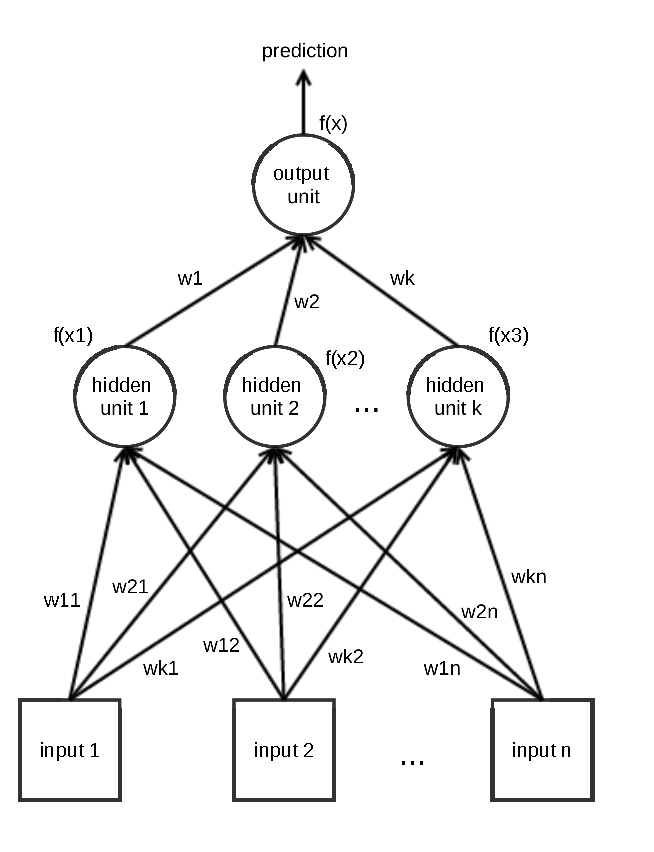
\includegraphics{images/method/mlp.eps}
\caption{An MLP with one hidden layer.}
\label{fig:mlp}

\end{figure}

MLPs can be trained in a number of ways, the most common of which is
\textit{backpropagation}. Suppose that we have the network above, with one
input, hidden and output layer respectively. From the perceptron learning
algorithm, we can update the weights of the hidden neurons leading to the
output neuron, but we do not know what the outputs of these hidden neurons are.
Backpropagation solves this problem by updating the weights of the various
connections to the hidden units based on the strength of the unit's
contribution to the final prediction, using a mathematical optimisation
algorithm called \textit{gradient descent}. This requires taking derivatives,
so the threshold function we used for the perceptron is usually replaced with
the sigmoid function $f(x) = \frac{1}{1+e^{-x}}$. We also define an error
function $E=\frac{1}{2}(\text{actual} - \text{predicted})^2$ -- the one most
commonly used -- which is
minimised in the gradient descent process. Updating the weights for each
connection in the network now involves finding the value of the derivative,
multiplying it by a small constant between 0 and 1 called the
\textit{learning rate}, and subtracting this value from the current weight
value, until the minimum for the error function is reached. Note that the
error function is quadratic, so it is guaranteed to have a minimum. The
updating of the weights is continued until the minimum is reached or if we
are ``close enough'' to the minimum.

It can be shown that MLPs with a single hidden layer are powerful enough to
model any continuous function, provided there are enough neurons in that
hidden layer \cite{Hand2001}. However, as they must iterate over the entire
data set many times, and due to the sometimes slow convergence of gradient
descent, MLPs are often slower to train than other learning algorithms we
have described, such as decision trees. We use them in this work on LOS
classification as we would like to see how they perform in modelling the
complex relationships between various medical attributes.

\section{Summary}
In this chapter we have outlined all of the learning algorithms that we will
be evaluating with respect to our classification problem, from the simple
Zero-R and 1R to Na\"{i}ve Bayes, decision trees, logistic regression,
$k$-nearest neighbour (and extensions K* and Ranked Distance), to the more
sophisticated support vector machines and multi-layer perceptrons. The reason
for our inclusion of so many algorithms is two-fold. Firstly, many of
these algorithms have not been extensively applied in various medical settings
to the problem of LOS prediction. Using a wide range of algorithms from various
paradigms will enable us to see what algorithms perform better than others.
Secondly, evaluating several classifiers will allow us to make comparisons
between different feature selection methods that are independent of the
classifier and give us more insight into the nature of the data set and of the
problem.
